\section{Problemas de asignación}

\subsection{Introducción}

En este tipo de problemas se trata de asignar, de la forma más eficiente, un conjunto de trabajos o tareas a una serie de 
máquinas o procesadores. Los procesadores pueden ser personas, vehículos, ordenadores,... Si se tienen $n$ tareas para asignar
a $m$ máquinas o procesadores, se supondrá que cada tarea debe ser asignada a una única máquina o procesador, es decir las 
tareas no pueden ser divididas.

\vspace*{2mm}

Asociando índices $i=1,\dots,m$ para las máquinas o procesadores y $j=1,\dots,n$ para las tareas, en los problemas de 
asignación se tienen variables binarias $x_{ij}$ que indican la asignación de la tarea $j$ a la máquina o procesador $i$.
Solo se puede asignar una tarea a una máquina o procesador al mismo tiempo, por lo que es necesaria una restricción del tipo
\[
    \sum_{i=1}^m x_{ij}=1 \quad j=1,\dots,n
\]
Además, existe un coste o tiempo de asignación para cada tarea y máquina $c_{ij}$. Dependiendo de si cada máquina puede
efectuar una única tarea o varias en el periodo considerado se obtienen diferentes problemas de asignación.

\subsection{Problema Clásico de Asignación}

En este tipo de problemas se supone, además de la restricción de asignación anterior, que cada máquina solo puede ejecutar 
una tarea en el periodo considerado. En el problema clásico de asignación el número de tareas $n$ coincide con el número de
máquinas o procesadores $m$, de forma que el model completo se formula como

\begin{alignat}{3}
    \text{minimizar:}   &   \sum_{i=1}^m\sum_{j=1}^n c_{ij}x_{ij}       \\
    \text{sujeto a:}    &   \sum_{i=1}^m x_{ij}=1 \quad j=1,\dots,n     \\
                        &   \sum_{j=1}^n x_{ij}=1 \quad i=1,\dots,m     \\
                        &   x_{ij} \in {0, 1} \quad i=1,\dots,m \quad j=1,\dots,n
\end{alignat}

Se puede apreciar que el Problema Clásico de Asignación coincide con el Problema de Transporte balanceado cuando $m=n$ y tanto
la oferta como la demanda total valen 1. Entonces, cualquier método de solución del problema de transporte puede aplicarse
también al Problema de Asignación.

\subsubsection{Métodos de solución}

\begin{itemize}
    \item La heurística greedy o de costo mínimo. En cada paso se toma $xij=1$ para la casilla $(i,j)$ de costo mínimo, y se
    elimina la fila y columna correspondiente, hasta completar la asignación. También se conoce como el algoritmo miope, pues
    solo ve de cerca.
    \item El método de penalización de Vogel. Funciona exactamente igual que en el Problema de Transporte. Para cada fila y 
    columna de la matriz de costos, se calcula una penalización (diferencia entre el segundo costo y el costo mínimo), se elige
    la fila o columna con penalización máxima, y se efectúa la asignación sobre el elemento mínimo de la fila o columna. 
    \item Método regret. Se trata de una versión del método de Volgel. en cada iteración se calcula la penalización o regret 
    solo para cada tarea, se elige la tarea con penalización máxima y se asigna a la máquina de costo mínimo aún sin asignar.
    \item El método húngaro. Es un algoritmo específico para el problema clásico de asignación, en el que se garantiza la 
    resolución óptima del problema.
    \item Por Simplex. Se formula el problema con variables $x_{ij}\geq 0$ y por la propiedad de integridad de los problemas de
    redes es seguro obtener soluciones $x_{ij}\in {0,1}$.
\end{itemize}

Como en los anteriores problemas, es posible mejorar la solución mediante búsqueda local. Para este problema definimos el 
entorno de la solución mediante intercambios de $k$ asignaciones. Se escogen $k$ tareas al azar y se intercambian las 
máquinas o procesadores asignadas a cada una mediante permutaciones. Es muy costoso computacionalmente pues su complejidad
es $O(n!)$.

\subsection{Problema de Asignación Generalizada (GAP)}

En este problema se supone que cada máquina puede ejecutar varias tareas, pero hay un tiempo máximo $b_i$ para la máquina o 
procesador $i=1,\dots,m$ que no puede superarse. Para ello hacen falta tanto los costes $c_{ij}$ como los tiempos $t_{ij}$ de
ejecución de una tarea $j$ para la máquina o procesador $i$. El modelo se formula tal que

\begin{alignat}{3}
    \text{minimizar:}   &   \sum_{i=1}^m\sum_{j=1}^n c_{ij}x_{ij}               \\
    \text{sujeto a:}    &   \sum_{i=1}^m x_{ij}=1 \quad j=1,\dots,n             \\
                        &   \sum_{j=1}^n t_{ij}x_{ij}\leq b_i \quad i=1,\dots,m \\
                        &   x_{ij} \in {0, 1} \quad i=1,\dots,m \quad j=1,\dots,n
\end{alignat}

En otras ocasiones, el problema GAP tien un formato de maximización, y en este caso los coeficientes $c_{ij}$ indican
rendimientos y las restricciones de tiempos disponibles son restricciones de recursos.

\subsubsection{Métodos de solución}

En esta ocasión el problema no puede ser resuelto mediante Simplex pues no se trata de un problema de redes y podrían obtenerse
soluciones fraccionarias. Se pueden aplicar tanto el algoritmo miope como el métodod de Vogel, aunque suelen fallar en 
encontrar una solución factible pues como $n$ puede ser distinto de $m$ podríamos ``saturar'' las máquinas o procesadores sin
llegar a asignar todas las tareas. 

\newpage

El Algoritmo de Martello y Toth es el método de penalizaciones aplicado al problema GAP. Llamemos $N=\{1,\dots,n\}$ al conjunto
de tareas, $M=\{1,\dots,m\}$ al conjunto de máquinas o procesadores, $U\subseteq N$ al conjunto de tareas aún sin asignar, $na$
al número de tareas asignadasm $\overline{b}_i=b_i$, $i=1,\dots,m$ la capacidad residual de la máquina $i$, $y_j$ la máquina
asignada a la tarea $j$, $z$ el valor objeto de la solución heurística y $feas$ una variable para indicar si se obtiene una
solución factible ($feas=1$) o no ($feas=0$).

\begin{enumerate}
    \item \textbf{Etapa 1, Inicialización}. Se asignan $U=\emptyset$, $na=0$, $\overline{b}_i=b_i\; i=1,\dots,m$, $z=0$ y 
    $feas=1$.
    \item \textbf{Etapa 2, Finalización}. Si $feas=1$ y $na=n$ se termina con una solución factible con valor $z$. Si $feas=0$
    se termina pero no se ha podido construir una solución factible. Si $feas=1$ y $na<n$ se va a la etapa 2.
    \item \textbf{Etapa 3, Penalizaciones}. Para cada tarea aún no asignada $j\in U$ sea 
    $F_j=\{i\in M:t_{ij}\leq\overline{b}_i\}$ y sea $nk_j = |F_j|$, es decir, el número de máqinas con capacidad de ejecutar la
    tarea $j$. Si $nk_j=0$ es imposible dar una solución factible por lo que $feas=0$ y termina la etapa. Si $nk_j=1$ se toma
    la penalización $p_j=\infty$. Si $nk_j\geq 2$ entonces $p_j=c_{(2)j}-c_{(1)j}$ para $c_{ij}:i\in F_j$. Entonces se encuentra
    la tarea $j^*$ con penalización $p_j$ máxima y se asigna a la máquina $i^*\in F_j$ con menor coeficiente $c_{ij}$, tomando
    $y_{j^*}=i^*$, $z=z+c_{i^*j^*}$, $\overline{b}_{i^*}=\overline{b}_{i^*}-t_{i^*j^*}$ y $na=na+1$. Volvemos a la etapa 2.
\end{enumerate}

\subsubsection{Búsqueda local}

Para aplicar la búsqueda local hace falta definir el entorno de una solución. Para el problema GAP se destacan dos tipos de
entornos

\begin{itemize}
    \item Entorno Shift. También llamado entorno de cambio, dada la asignación actual un movimiento shift consiste en cambiar
    la asignación de la tarea $j'$ a otra máquina o procesador diferente.
    \item Entorno Swap. También llamado entorno de intercambio, dada la asignación actual un movimiento swap consiste en 
    intercambiar la asignación de dos tareas $j_1$ y $j_2$.
\end{itemize}

\begin{figure}[h!]
    \centering
    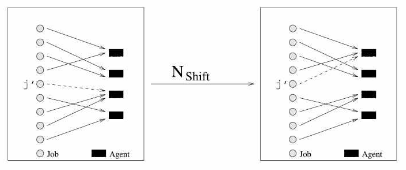
\includegraphics[width=0.7\textwidth]{img/EntornoShift.png}
    \caption{Ejemplo de movimiento shift}
\end{figure}

\newpage

\begin{figure}[h!]
    \centering
    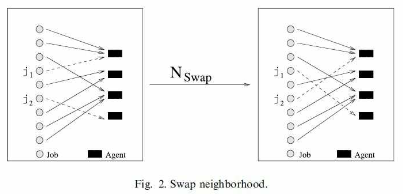
\includegraphics[width=0.7\textwidth]{img/EntornoSwap.png}
    \caption{Ejemplo de movimiento swap}
\end{figure}

\noindent Para obtener una solución mediante busqueda se puede aplicar un único tipo de entorno a la solución ofrecida por el
método Martello-Toth o mezclarlos de forma secuencial o, mejor aún, con un método de descenso VNS.

\subsection{Objetivos minimax}

En algunas ocasiones, tanto en el problema de asignación clásico como en el generalizado, en vez de minimizar el tiempo o 
coste total incurrido al asignar todas las tareas, puede interesar minimizar el tiempo máximo de ejecución entre todas las 
tareas, o bien el tiempo máximo de ejecución entre todas las máquinas. Este segundo objetivo es conocido como 
\textit{makespam}. Aunque ambos objetivos son no lineales, se pueden convertir facilmente en problemas lineales.

\vspace*{2mm}

Para el primer objetivo basta con añadir una variable $w\geq 0$ indicando el tiempo máximo y añadir las restricciones
\[
    \sum_{i=1}^m t_{ij}x_{ij}\leq w \quad j=1,\dots,n
\]

Para el segundo objetivo basta con, de nuevo,  añadir una variable $w\geq 0$ indicando el tiempo máximo y añadir las 
restriciones
\[
    \sum_{j=1}^n t_{ij}x_{ij}\leq w \quad i=1,\dots,m
\]